\documentclass[12pt]{article}
    \title{\textbf{CAP6635 Project Report 1}}
    \author{William L. Thomson Jr.}
    \date{Spring Semester 2024}

    \usepackage{enumitem}
    \usepackage{float}
    \usepackage{hyperref}
    \usepackage{graphicx}
    \usepackage[T1]{fontenc}
    \usepackage{titlesec}
    \usepackage[tmargin=1in,lmargin=1in,rmargin=1in]{geometry}

    \addtolength{\topmargin}{-3cm}
    \addtolength{\textheight}{3cm}
    \hypersetup{
		colorlinks=true,
		linkcolor=blue,
		urlcolor=blue
    }
    \titleformat{\section}{\normalfont\bfseries}{\thesection}{0.5em}{}
    \titlespacing\section{0pt}{12pt plus 4pt minus 8pt}{4pt plus 2pt minus 8pt}
\begin{document}

\maketitle

\vspace{-2em}

\section{Research}
\indent \indent Initial research done thus far is mostly in understanding the paper implementation and
how we are deviating from that. We will not be changing the start location, as they change the start location when a new goal is set. We will also not be changing the goal location.
Pending further research and the ultimate solution, we may or may not be returning back
to the original path as determined by IRRT*.

It is not clear at this time to what extent we will be re-wiring the tree, pruning any leaf
nodes and adding others. This might be done as part of Tangent Bug implementation, and/or
after the fact with the new route taken, either back to original or entirely new path to 
goal, which might entail another round of IRRT*.

\section{Plan}
The current plan of action is as follows:
\begin{description}[style=multiline,leftmargin=8em]
\itemsep0em
\item[IRRT*] Run IRRT* to determine the path to goal with random obstacles
\item[New Obstacle] A new obstacle is randomly added/detected as the path is being traversed,
					the path that IRRT* identified, the new obstacle intersects that path.
\item[Collision Zone] The path will be traversed till the obstacle enters a collision zone,
                      which might require adding a new node, as the collision zone might
                      be smaller than the distance from the previous node to the new obstacle
\item[Tangent Bug] Use Tangent Bug to go around the obstacle at some distance, to some next point
\item[To Be Decided] From Tangent Bug it has yet to be decided the method used to either return
					 to the initial path from IRRT* or to re-route to a shorter path to the goal
					 via some method to be decided.
\end{description}

\section{Progress}
\indent \indent Initial prototype code has been written using \href{https://github.com/AtsushiSakai/PythonRobotics/tree/master/PathPlanning/InformedRRTStar}{PythonRobotics implementation of IRRT*}, with randomized
start, goal, and obstacles. After IRRT* is run, a obstacle is randomly added long the path
as seen in Figure \ref{figure1}. Alternative prototyping was also done with a new random goal, per the paper implementation as seen in Figure \ref{figure2} and \ref{figure3}, but we will not be exploring that approach. Although, it does present an additional challenge, if that new obstacle causes a new goal, \emph{e.g.}  door closed obstacle, or other none traversal.

\section{What's next}
\indent \indent The next step is to code in a variable collision zone, and code for detecting the nearest node to the newly detected object, and potentially, creating another outside the collision zone distance, that will be used as a buffer distance for Tangent Bug to remain that distance away from the
obstacle.

\vspace{1em}

\newpage
\addtolength{\topmargin}{2cm}


\begin{figure}[H]
\begin{center}
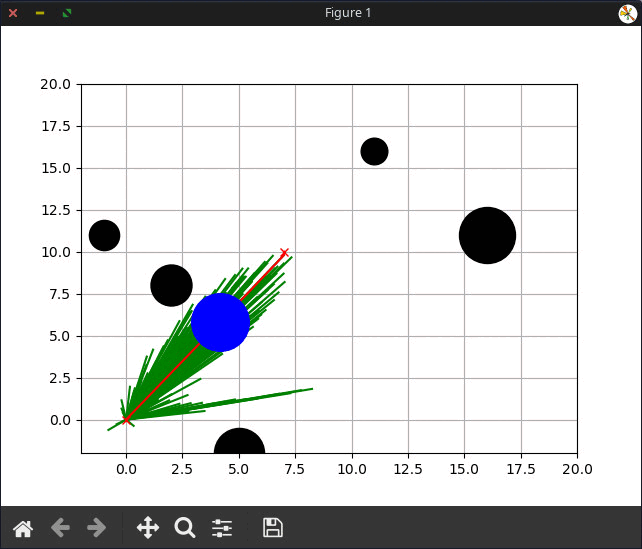
\includegraphics[scale=0.35]{screenshots/shot1_random_obstacle}
\caption{Screenshot of random obstacle on IRRT* path}
\label{figure1}
\end{center}
\end{figure}

\vspace{-2em}

\begin{figure}[H]
\begin{center}
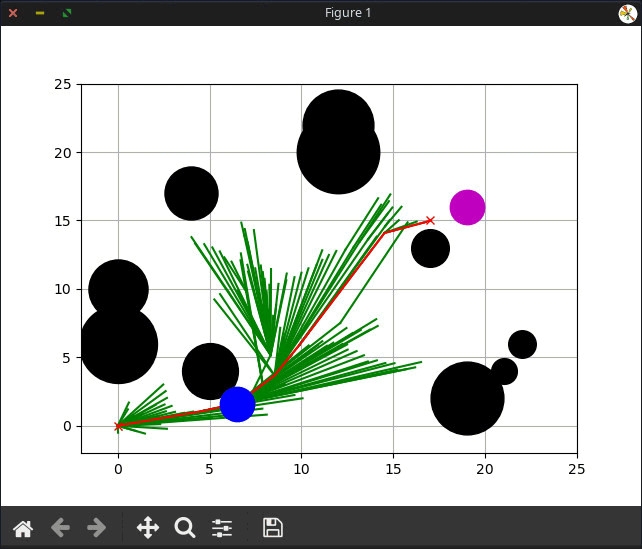
\includegraphics[scale=0.35]{screenshots/shot2_new_goal}
\caption{Screenshot of random new goal on IRRT* path}
\label{figure2}
\end{center}

\vspace{-2em}

\end{figure}
\begin{figure}[H]
\begin{center}
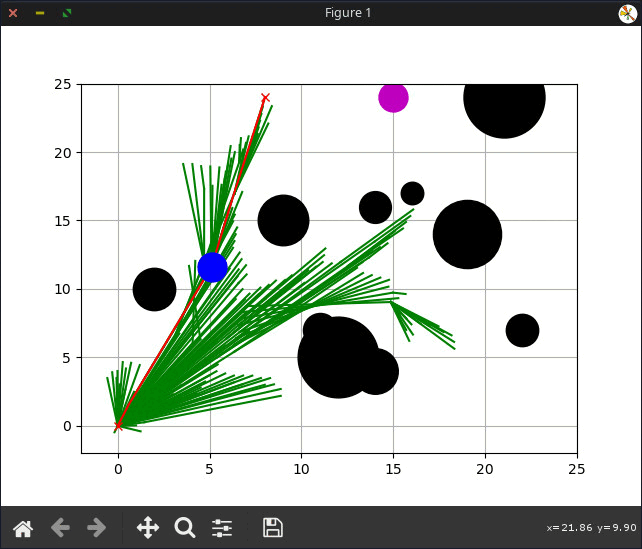
\includegraphics[scale=0.35]{screenshots/shot3_new_goal}
\caption{Screenshot of random new goal on IRRT* path}
\label{figure3}
\end{center}
\end{figure}

\vspace{-3em}

\end{document}

